\documentclass{article}
\usepackage[utf8]{inputenc}

\title{Team 39 Final Report: Fluid Simulation}
\author{Yekang Chang, Jie Zeng, Silu Chu, Liang Yang}
% \date{April 2024}
\usepackage{hyperref}
\usepackage{listings}
\newcommand{\cmdname}[1]{\texttt{#1}}
\newcommand\footurl[1]{\footnote{\url{#1}}}
\newcommand\urllink[2]{#1\footurl{#2}}
\newcommand\foothref[3]{#1\footnote{\href{#2}{#3}}}
\usepackage{upquote}
\usepackage{graphicx} % For including graphics
\usepackage{subcaption} % For creating subfigures

\begin{document}

\maketitle
% summarize what you have accomplished, preliminary results, reflect on progress relative to your plan, and update your work plan as appropriate

The demo video link is published at \url{https://drive.google.com/file/d/1LMpycsC-qMtw3NhOV_5KMmnzrUuYepJs/view?usp=drive_link}.

\section{Abstract}

% A paragraph summary of the entire project.

\hspace{1em} In this project, our group, building on a tutorial \foothref{\textit{Simulating Fluids}}{https://www.youtube.com/watch?v=rSKMYc1CQHE&t=1396s}{\texttt{https://www.youtube.com/watch?v=rSKMYc1CQHE\&t=1396s}},
  will simulate the fluid within a tank, and then we will simulate the real-case scenario when a ball falls into and interacts with the fluid (which many liquid drops will bounce out).We have implemented the fluid in a more vivid and real way, as well as the simulation of the interaction after the ball drops and fluid particle splashed. 

\section{Technical approach}
% - A 1-2 page summary of your technical approach, techniques used, algorithms implemented, etc. (use references to papers or other resources for further detail). Highlight how your approach varied from the references used (did you implement a subset, or did you change or enhance anything), the unique decisions you made and why.
% - A description of problems encountered and how you tackled them.
% - A description of lessons learned.

\subsection{Spawner, Interaction between particles}
 \hspace{1em} In our water simulation project, the Spawner3D class is crucial for generating the initial set of particles that populate the simulation space. This section will cover how the Spawner3D class functions and the key interactions between particles that drive the realistic simulation of fluids.

\subsubsection{Spawner3D Class}
 \hspace{1em} The Spawner3D class initializes particles within a cubic volume, centered at a specified centre and sized according to size. The numParticlesPerAxis defines how densely particles are placed along each axis, resulting in a total of $numParticlesPerAxis^3$ particles. Properties such as initialVel set the initial velocity of particles, and jitterStrength introduces randomness to particle placement, enhancing realism by preventing uniform spacing.

 The 'GetSpawnData' Method computes the initial positions and velocities for each particle. It employs a three-dimensional nested loop, iterating over each axis to calculate the position of particles based on their relative location in the grid. The addition of a random jitter (UnityEngine.Random.insideUnitSphere * jitterStrength) to each particle's position helps simulate a more natural particle distribution. Each particle is assigned the initial velocity specified by initialVel.

\subsubsection{Interaction between Particles}
 \hspace{1em} The "Simulation3D" class manages the simulation's lifecycle, handling updates per frame and integrating physical interactions between particles. It employs simulation settings like "timeScale" for controlling simulation speed and "fixedTimeStep" to toggle between fixed and variable time steps. Physics properties such as "gravity" and "collisionDamping" affect how particles interact with gravity and how they respond to collisions.

 Particle interactions are governed by compute shaders that calculate physical forces acting on each particle. This includes forces due to pressure, viscosity, and external influences like gravity. The system uses spatial hashing, implemented in the compute shader, to efficiently manage and query particle neighborhoods, essential for scaling the simulation to a large number of particles.

 The "FluidSim3D.compute" shader script updates particle states including position and velocity. The shader functions handle different aspects of the simulation: "UpdatePositions" updates particle positions based on velocities, "ResolveCollisions" ensures particles remain within bounds by adjusting positions and velocities upon collisions, and "ResolveSphereCollision" dynamically adjusts interactions when particles collide with a moving sphere.

\subsection{Performance Improvement for Large Number of Particles}
\hspace{1em} After the simulation model for particles and the interaction between them are established, we need to elevate the performance when we need to simulate large number of particles, otherwise the animation will not go smooth. We do the performance improvement in the process of calculating densities and pressure forces for a certain particle, which we avoid looping over all particles that lie outside the smoothing radius, as they contribute nothing to the calculation.

\subsubsection{Optimize Particle Lookup}

\hspace{1em}To achieve this, we partition the space of particles into grids, with certain number of particles lying inside each grid cells, and the size of the grid cells is set to be the "smoothing radius". As a result, we only need to consider particles lying inside the 3*3 grids of cells around the center of circle when calculating the interaction forces for a certain particle. 

But we want to convert the whole simulation to a compute shader at some point, and on the GPU we do need  to specify ahead of time how much memory we’re going to use. A GPU-friendly approach is adopted from the  \foothref{\textit{paper}}{https://web.archive.org/web/20140725014123/https://docs.nvidia.com/cuda/samples/5\_Simulations/particles/doc/particles.pdf}{\texttt{https://web.archive.org/web/20140725014123/https://docs.nvidia.com/cuda/sam\-ples/5\_Simulations/particles/doc/particles.pdf}}, so that we don’t need to know the dimensions of the grid ahead of time, meaning that particles can travel anywhere in the world, and it’ll still work. We first create a single array with size to be maximum number of particles within the grid map. 

For each particle in the array, we calculate the coordinate of the grid cell it is in. We need to do hashing in order to turn the coodinate of the cell (within the grid) into a single number, and also get the key of this certain coordinate ("cell key"), for example, do modulo by the size of array. Then, each particle within the array is associated with a "cell key" it is in. To efficiently loop over the array, we want to sort the array based on "cell key" in order to let the particles within the same grid cell (same "cell key") staying next to each other in the array. The new sorted array is called \textit{spatialLookup}. Another array called \textit{startIndices} is established, with element at position \textit{i} to be the index of first element in array \textit{spatialLookup} that is in "cell key" with value \textit{i}. We can use the array \textit{startIndices} to quickly locate all the particles in \textit{spatialLookup} that we are interested in (particles storing in a particular grid cell). To avoid the problem of locating particles in different grid cells but hash to the same "cell key", we will do the distance checking for 2 cells to ensure they are exactly in the same grid cell and inside the smoothing radius.  

The \textit{UpdateSpatialLookup()} function will update the \textit{spatialLookup} array whenever the points moved, which include creating the \textit{spatialLookup} using hashing, sorting it based on cell key, and generate the \textit{startIndices}. The \textit{ForeachPointWithinRadius()} function will find all of the (particle) points within the smoothing radius of a certain particle. It will loop over all the 3*3 grid cells around the particle and process the particle information in these grid cells. 

\subsubsection{Particle Movement Simulation Improvement}

Now, the simulation of large number of particles can be done smoothly, but it is totally in chaos(random movements). We can optimize this by predicting the next position of particle based on current velocity and external forces , then use the predicted position for calculating \textit{densities} and \textit{pressureForce} after \textit{deltaTime}. In the particle rendering code, we visualize the speed of particle with color.


\subsection{Bouncing Sphere}
 \hspace{1em} We added one sphere into our scenario and it will fall from some height and splash the fluid particles we implemented. When it collides with the floor, it will also be applied with an opposite force which forces the sphere to bounce.

\subsubsection{Bouncing Sphere Interacts with Particles}
 \hspace{1em} In one GPU-processed Unity script file \textit{Fluid3d.compute}, we added one function \textit{ResolveSphereCollision} to handle the interaction between sphere and particles. When the sphere is in motion, its effective collision radius can increase based on its speed, enhancing the realism of interactions by accounting for motion blur effects. To be consistent with our intuition, the sphere would be applied with force by every fluid surrounding it, so we basically achieve this by converting it into interaction on three dimensions of this sphere. On the other hand, as the sphere encounters particles, it applies a force that pushes them away, proportional to both the penetration depth and the sphere's velocity. 




\subsubsection{Bouncing Sphere Interacts with Floor}
 \hspace{1em} Additionally, the sphere's collision with the boundaries of its container is managed by adjusting its position and inverting its velocity upon contact with the edges, damping its speed to simulate energy loss. If the sphere's velocity falls below a threshold, it is effectively halted to prevent unnecessary computations when the motion is negligible.





\subsection{Improving Shader}
\hspace{1em} With the original shader, the particles display like individual balls, which was not we wanted. So we made some edition to make them seem more like fluid.
\subsubsection{Transparent Rendering}
\hspace{1em} We considered introducing transparent rendering and changing the alpha value of the particles according to their speed, and it looks good because the area with less particles look more transparent. We changed the render queue into \textit{Transparent} and used the Blend command \textit{Blend SrcAlpha OneMinusSrcAlpha} in ShaderLab to enable transparent rendering.
\subsubsection{Illumination}
\hspace{1em} We also want to show the effect of light. Because the particles are created after the programme started, they cannot be rendered by the light in the scene. So we have to calculate the light in the shader. We then referenced the shader part in assignment 4 to add illumination to the fluid. We chose Blinn-Phong shading, calculating the diffuse and mirror reflection. We also adjusted the colour map to make it more close to real water.

\section{Results}

\hspace{1em} The below three figures are captured from our current preliminary simulation results. We have done a demo-simulation of the fluid. In this scenario, the fluid - simulated in the form of liquid drops, falls down from a "spawner" and spreads across the container tank. 

We then do a preliminary simulation of the ball that falls into the pool and interacts with the liquid drops. Ball falls at different velocities will lead to different results of interaction with fluid. For example, when the ball falls from higher places or large velocity, more liquid drops will be splashed out, and will be splashed higher. 

\begin{figure}[h]
    \centering
    \begin{subfigure}[b]{0.33\textwidth}
        \centering
        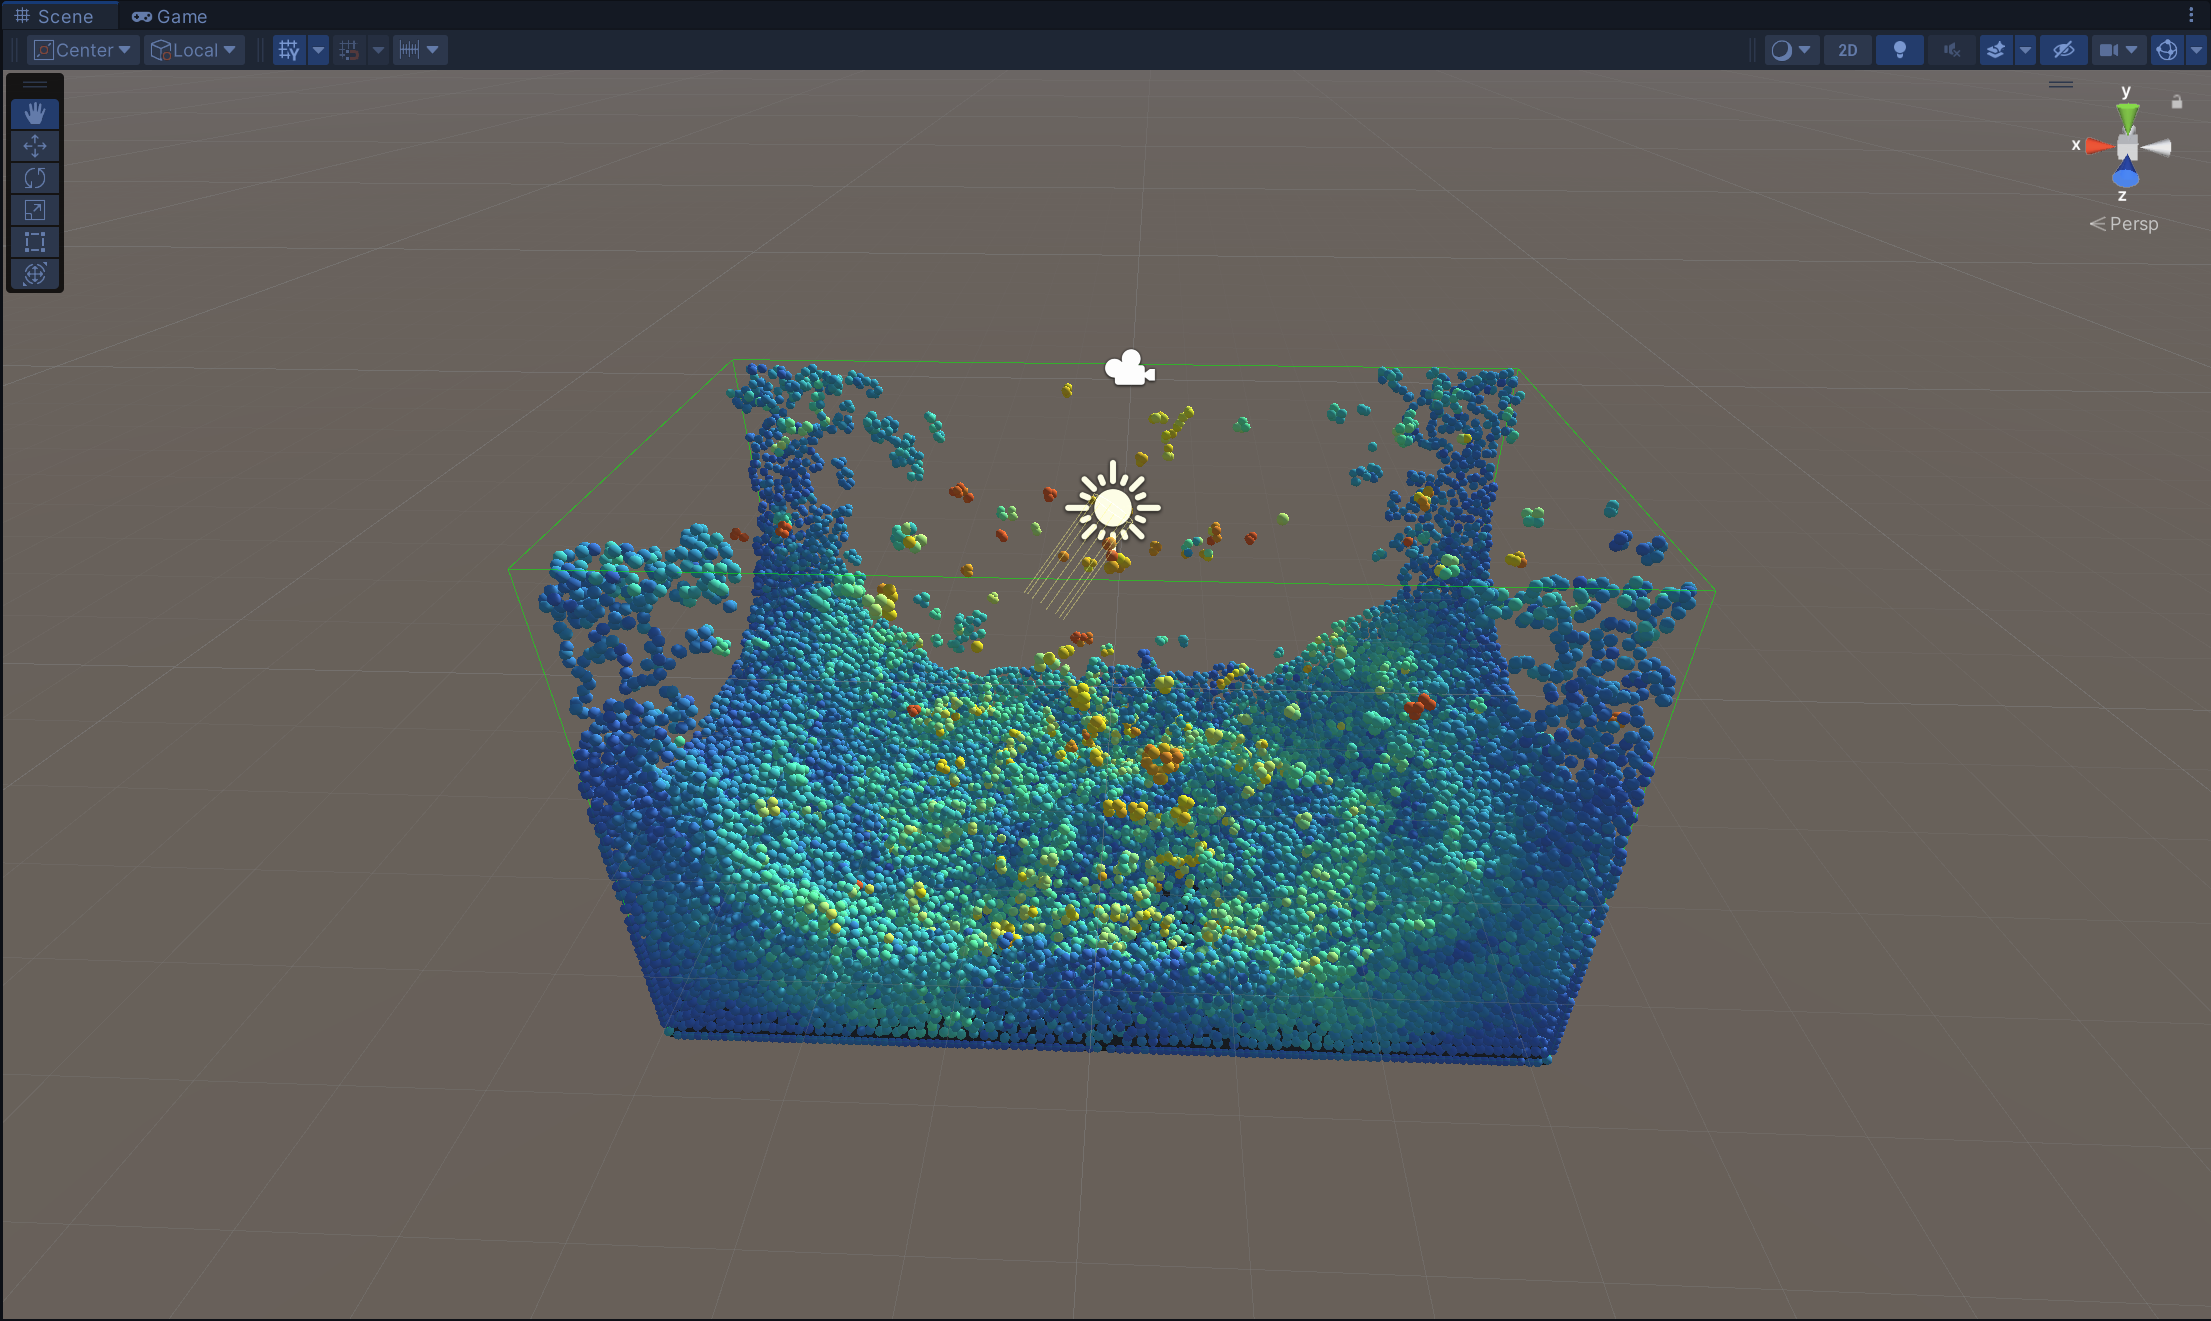
\includegraphics[width=0.9\textwidth]{water_model_mode.png}
        \caption{Water in Scene View}
        \label{fig:higher_velocity}
    \end{subfigure}%
    \hfill % Adds horizontal space between the subfigures
    \begin{subfigure}[b]{0.33\textwidth}
        \centering
        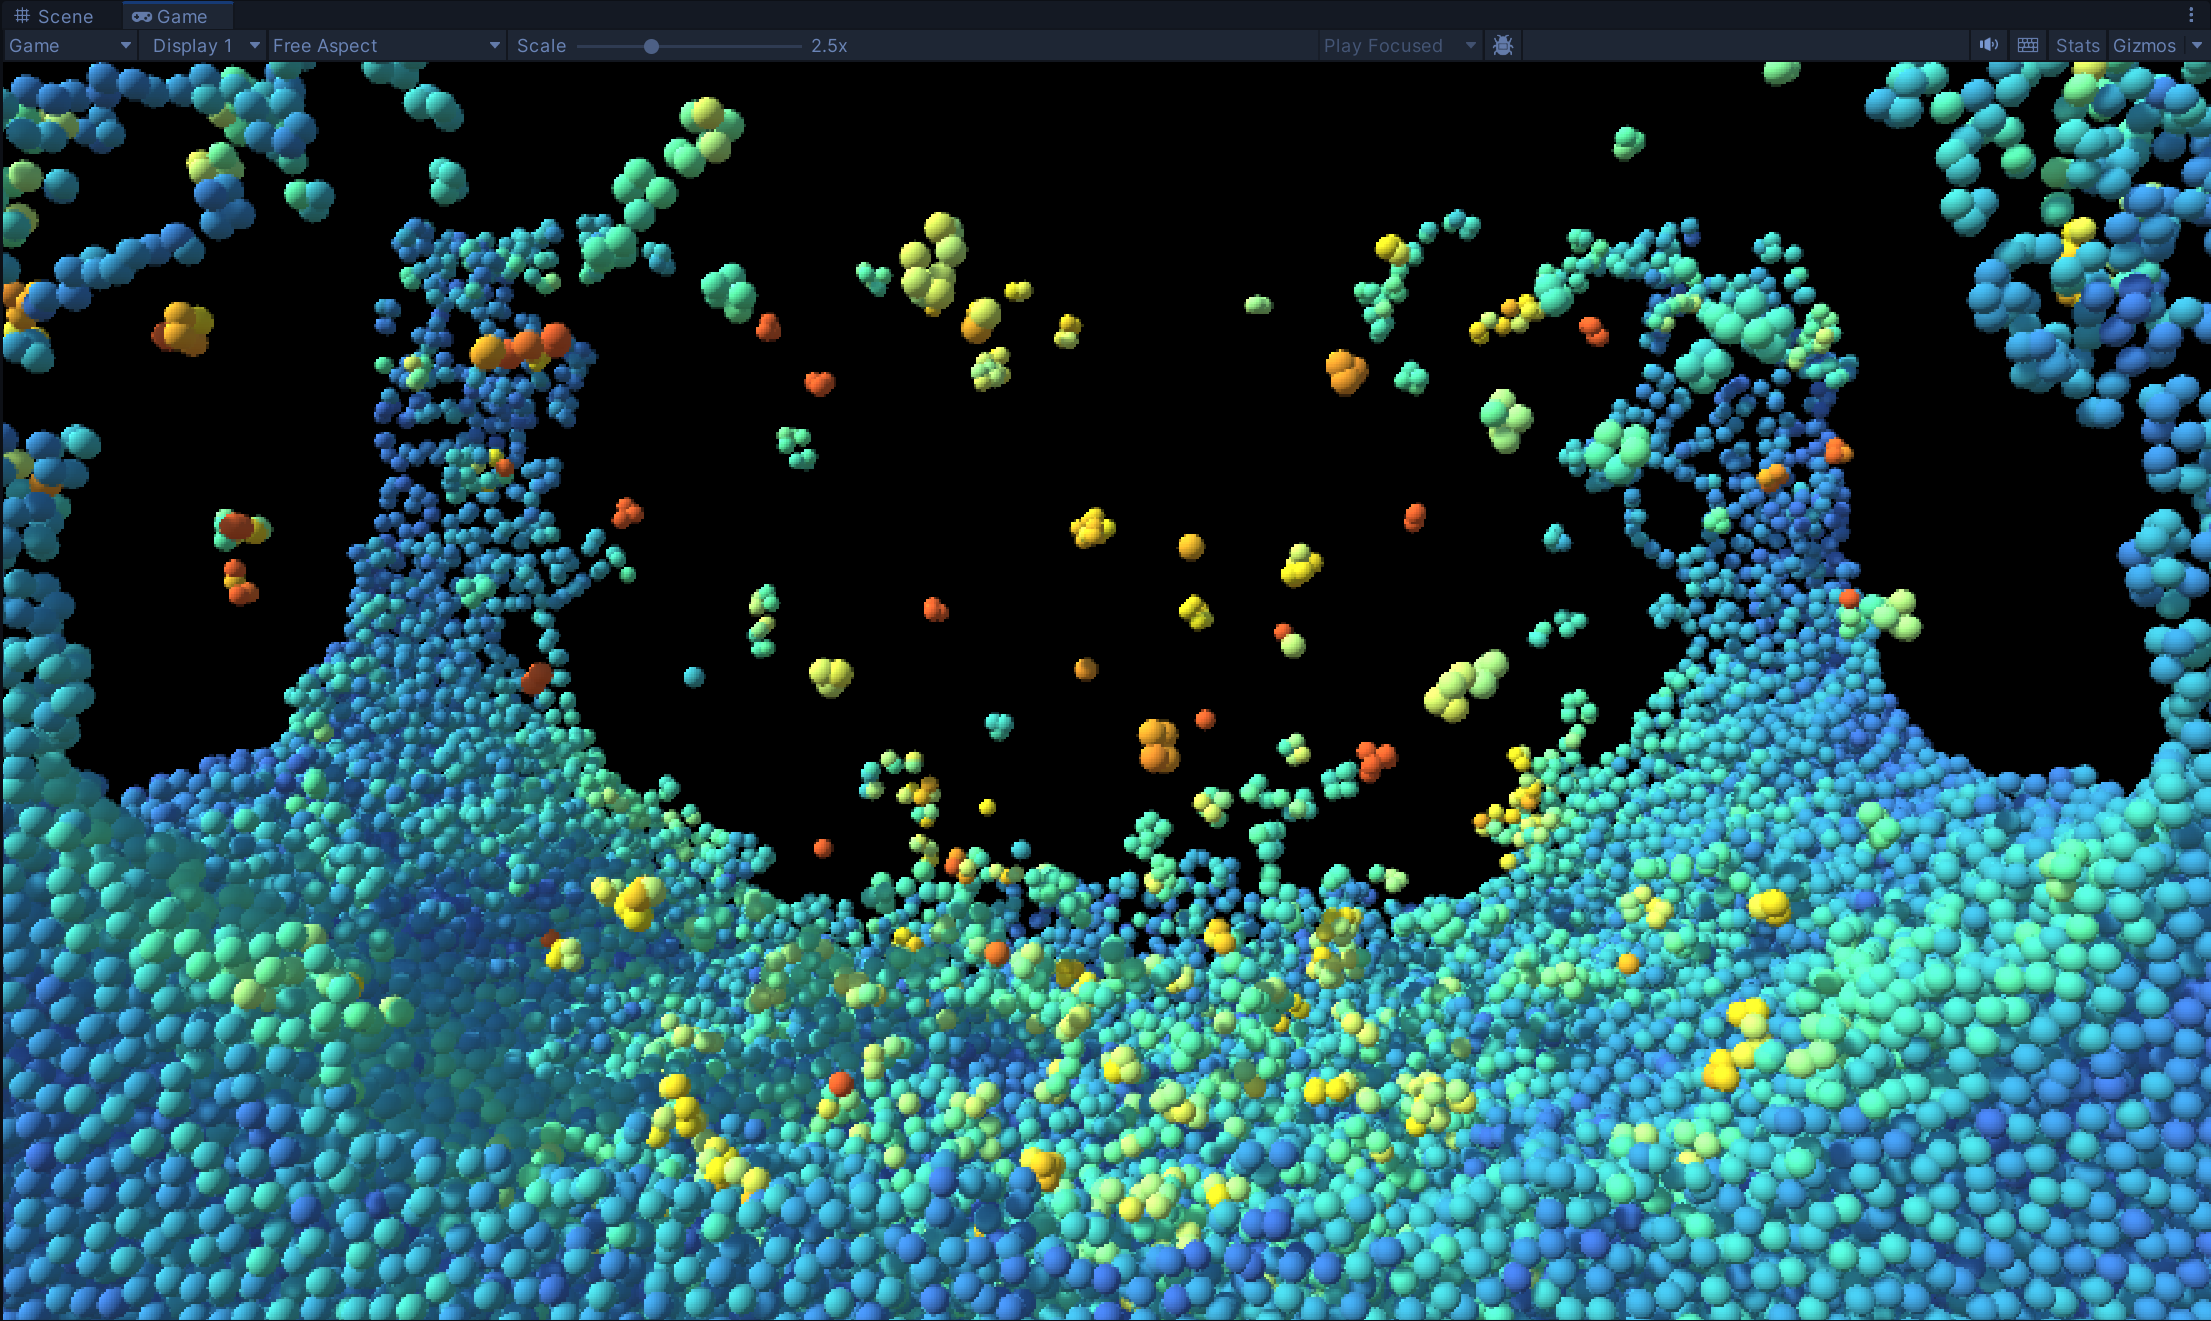
\includegraphics[width=0.9\textwidth]{water_game_mode.png}
        \caption{Water in Game Mode}
        \label{fig:lower_velocity}
    \end{subfigure}
        \begin{subfigure}[b]{0.33\textwidth}
        \centering
        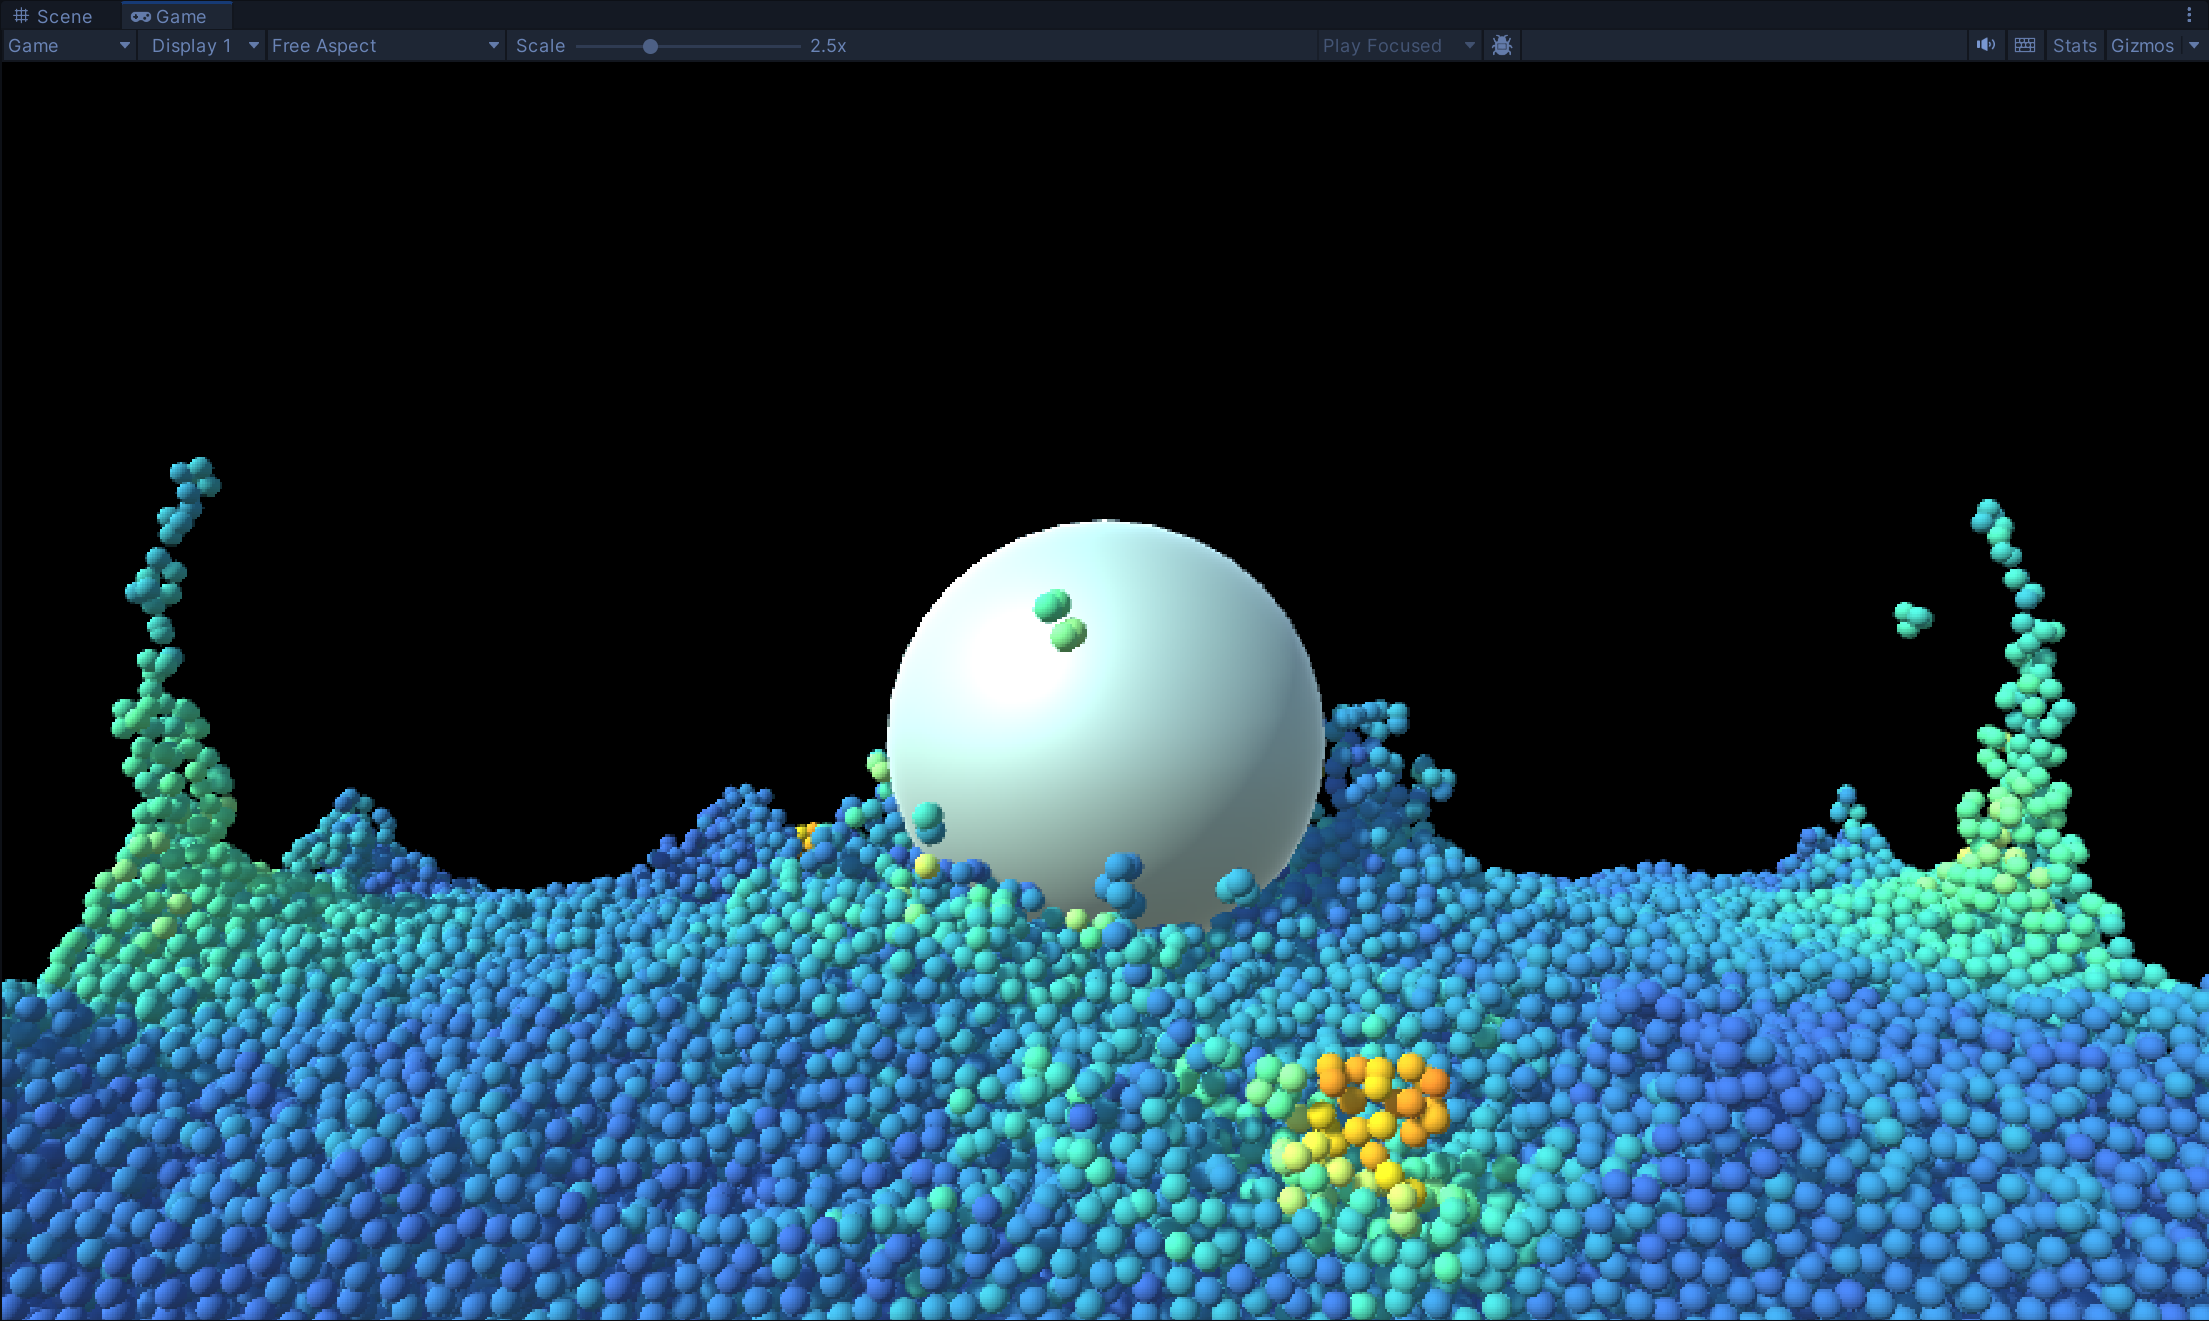
\includegraphics[width=0.9\textwidth]{ball_water.png}
        \caption{Ball drops in Water}
        \label{fig:lower_velocity}
    \end{subfigure}
\end{figure}

\section{References}
\begin{itemize}
    \item \url{https://web.archive.org/web/20140725014123/https://docs.nvidia.com/cuda/s\-amples/5_Simulations/particles/doc/particles.pdf}
    \item 
    \url{https://www.youtube.com/watch?v=rSKMYc1CQHE&t=1396s}
\end{itemize}


\section{Contributions Distribution}
\begin{itemize}
    \item Jie Zeng: Demo Video; Implementation of Sphere in this simulation; Organizing group meeting and process scheduling.
    \item Yeknag Chang: resources collection, implementation of water particles, and parameters tuning for shading.
    \item Silu Chu: 
    \item Liang Yang: resources collection, parameters tuning for shading and coloring, writing the milestone and final report website
\end{itemize}
    


% \section{Reflection}
%  The above figures are preliminary simulation demos for the fluid and its interaction with the ball. More refinement is needed, for example, as seen in the figure, the scenario when liquid drops splashed out is not real. 
% \noindent In addition, we current simulate the fluid in the form of discrete liquid drops, just like those "ocean balls" in children's amusement parks. We will further make the simulation of fluid more real.

% Figure 3: water with tuned parameters



% \section{Introduction}

% \urllink{Overleaf}{https://www.overleaf.com/} is popular online \LaTeX{}
% editor. It can generate PDF files 
% without need to install a local \TeX{} distribution. Unfortunatelly, it doesn't
% support conversion to HTML out of the box. To get the HTML version of the
% document, we must use some tricks.

% There are many tools that support the conversion from \LaTeX{} to HTML, each of
% them use a different approach. I am a developer of
% \urllink{\TeX4ht}{https://tug.org/tex4ht/}, so I will present solution that
% uses this tool. 

% \TeX4ht uses \TeX{} for the actual conversion. It loads special configuration
% files for internal \LaTeX{} code or for the used packages. These configuration
% files patch commands with special instructions that insert HTML (or other
% supported formats). Because it uses \TeX{} for the actual conversion, it
% supports custom commands. It also supports font changing commands, so  it
% doesn't need custom configurations in many cases.

% The first method that use \TeX4ht for the conversion was presented by LianTze
% Lim. It uses a custom build file for
% \urllink{Latexmk}{https://www.overleaf.com/latex/examples/testing-html-export-with-tex4ht/rqcknjvwyyry} 
% that calls \TeX4ht. The downside is that the generated HTML file is not easilly accessible.  

% To make the conversion easier, I've set up \urllink{Docker image}{https://hub.docker.com/repository/docker/michalh21/make4ht-docker/general} for \TeX4ht. 
% Thanks to \urllink{GitHub Actions}{https://help.github.com/en/actions/automating-your-workflow-with-github-actions/about-github-actions}, 
% it is possible to use this image for the conversion of the Overleaf document to HTML. 
% The generated files can be published on the web using Github Pages, where they can be automatically 
% updated on every document change. This document is an example of this setup.

% \section{Setup}

% \subsection{On Overleaf}

% First step is to sync your Overleaf project with your GitHub account, following \foothref{a guide on 
%   Overleaf}{https://www.overleaf.com/learn/how-to/How_do_I_connect_an_Overleaf_project_with_a_repo_on_GitHub,_GitLab_or_BitBucket\%3F}
% {\texttt{https://www.overleaf.com/learn/how-to/How\_do\_I\_connect\_an\_Overleaf\_project\_with\_a\allowbreak\_repo\_on\_GitHub,\_GitLab\_or\_BitBucket\%3F}}. 
% Don't forget to run the \cmdname{Sync -> GitHub} command from Overleaf main menu every time you had updated the document.

% \subsection{On GitHub}
% Next step is to configure actions in the Github project created for your
% document. Two steps are necessary -- first  one compiles the document to HTML
% using \TeX4ht, the second step publishes the generated HTML files on the Web
% using \urllink{GitHub Pages}{https://pages.github.com/}

% For the web publishing we  use the \verb|actions-gh-pages|
% \urllink{action}{https://github.com/peaceiris/actions-gh-pages}. 

% When the keys are set up, you can create the workflow file. Select the
% \cmdname{Actions} tab and click the \cmdname{Set up a workflow yourself}
% button. It will open an editor with a YAML file for the Action workflow.
% Replace it with the following content:

% % I am just testing if this command works in the container
% \AtEndEnvironment{lstlisting}{\relax}

% \begin{lstlisting}{yaml}
% name: CI
% on: [push]
% jobs:
%   build:
%     runs-on: ubuntu-latest
%     steps:
%     - uses: actions/checkout@v1
%     - name: Run make4ht
%       uses: docker://ghcr.io/michal-h21/make4ht-action:latest
%       env:
%         command: "make4ht -u -d out main.tex"
%     - name: Publish the web pages
%       uses:  peaceiris/actions-gh-pages@v3
%       with:
%         github_token: ${{ secrets.GITHUB_TOKEN }}
%         publish_dir: ./out
% \end{lstlisting}

% The important part of the configuration is the \cmdname{command} key. It
% contains the actual command used for the compilation. We use
% \urllink{Make4ht}{https://ctan.org/pkg/make4ht?lang=en}, build system for
% \TeX4ht.

% Command \verb|"make4ht -u -d out main.tex"| creates UTF-8 encoded HTML file
% from the \cmdname{main.tex} input file. The \texttt{-d} option specifies the
% output directory for the HTML files. This directory will be used for the web
% publishing and should be passed to the \verb|publish_dir| key in
% \textit{Publish the web pages} step.

% The web will be published at \url{https://yourgitubusename.github.io/project_name/main.html}. 
% \section{Links}
% \begin{itemize}
%     \item This document: \url{https://www.kodymirus.cz/overleaf-html-sample/main.html}
%     \item Source repository: \url{https://github.com/michal-h21/overleaf-html-sample} 
% \end{itemize}
 



\end{document}
